% !Mode::"TeX:UTF-8"
% !TEX encoding = UTF-8
\section{不动点迭代法}
不动点迭代法(Fixed Point Iteration)是数值计算中求解非线性方程普遍使用的方法,其基本的思想是逐次逼近。首先给定一个初始值,然后使用一个迭代公式,反复校正这个初值,直到满足预先给定的精度要求为止。
\subsection{不动点}
让我们先来看一下什么是不动点
\begin{thm}
  如果对于一个给定的函数$\varphi$,有$\varphi(x^*)=x^*$,那么就$x^*$叫做$\varphi$的不动点.
\end{thm}
如下图所示,\\
\begin{figure}[h]
  \centering
  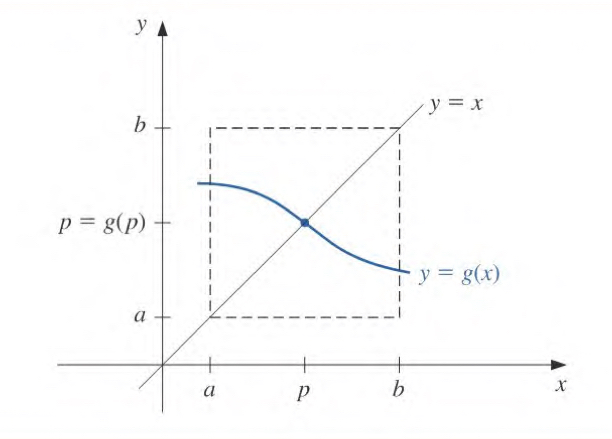
\includegraphics[scale=0.6]{fig1}
  \label{fig:fig1}
\end{figure}

则$p$即为$g(x)$的一个不动点.
\section{不动点迭代法的算法构造}
\subsection{基本思路}
已知方程$f(x)=0$在区间$[a,b]$内有唯一的实根$x^*$,将上式改写成等价形式$x=\varphi(x)$,取$x_0\in[a,b]$,用递推公式$x_{k+1}=\varphi(x_k)(k=0,1,2,\cdots)$,可以得到序列$x_0,x_1,\cdots$.如果当$k\rightarrow\infty$时,有极限$ \lim_{k\to\infty}x_k=x^*$,则称迭代法收敛于$x^*$,且$x^*=\varphi(x^*)$,则称$\varphi(x)为迭代函数$,$x_{k+1}=\varphi(x_k)$为迭代格式,${x_k}$为迭代序列;当$x_0\neq x^*$时,如果序列${x_k}$在$[a,b]$内无极限,则称迭代法发散。应当指出,为使迭代法有效,必须保证它的收敛性,一个发散的迭代过程,纵使迭代千万次,其结果也是毫无价值的。因而我们必须考虑迭代法的收敛性。
\subsection{收敛定理}
我们应当如何验证迭代格式的收敛性呢?这里就需要引入收敛定理。
\begin{thm}\label{t2.1}
设迭代函数$\varphi(x)$在$[a,b]$上有连续的一阶导数,且:

(1)当$x\in[a,b]$时,$a \leq \varphi(x)\leq b $.

(2)存在正数$q\leq1$(q为利普希茨常数),使对任意$x \in [a,b]$,有$\lvert \varphi'(x) \rvert \leq q<1 $.

则方程$x=\varphi(x)$在区间上存在唯一的根$x^*$,并且对任意初值$x_0\in [a,b]$,由迭代格式$x_{k+1}=\varphi(x_k)$所确定的序列${x_k}$均收敛于${x^*}$.
\end{thm}
\begin{proof}
设$x^*$为方程$x=\varphi(x)$的根,则由微分中值定理有
\begin{equation}
x^*-x_{k+1}=\varphi(x^*)-\varphi(x_k)={\varphi'}(\varepsilon)(x^*-x_k),
\end{equation}
式中$\varepsilon$是$x^*$与$x_k$中的某一点,于是有
\begin{equation}
\lvert x^*-x_{k+1}\rvert\leq q\lvert\ x^* - x_k \rvert.
\end{equation}
对此反复递推,对迭代误差$\varepsilon_k=\lvert x^* - x_k \rvert$,有
\begin{equation}
\varepsilon_k \leq q^k\varepsilon_0.
\end{equation}
由于$0<q<1$,因而$\varepsilon_k\rightarrow0(k\rightarrow\infty)$,即迭代法收敛.
\end{proof}
\begin{cor}\label{c2.1}
如果$\lvert{\varphi'}(x)\rvert>1$,则迭代格式$x_{k+1}=\varphi(x_k)$所确定的序列${x_k}$对任意初值$x_0\in [a,b]$发散.
\end{cor}
若存在$x^*$的某个邻域$I={x:\lvert x-x^* \rvert\leq\delta}$,使得迭代过程$x_{k+1}=\varphi(x_k)$对于任意初值$x_0\in I$收敛,则称迭代过程$x_{k+1}=\varphi(x_k)$在根$x^*$的邻近具有局部收敛性.
\begin{thm}\label{t2.2}
设$\varphi(x)$在$x=\varphi(x)$的根$x^*$的邻近有连续的一阶导数,且成立$\lvert {\varphi'}<1 \rvert$,则迭代过程$x_{k+1}=\varphi(x_k)$在根$x^*$附近具有局部收敛性。
\end{thm}
\begin{proof}
由于$\lvert {\varphi'}(x^*) \rvert < 1$,故存在充分小的邻域$I={x:\lvert x-x^* \rvert\leq\delta}$,使得$\lvert {\varphi'} \leq q <1\rvert$成立.这里q为某个常数.据微分中值定理,有
\begin{equation}
\varphi(x)-\varphi(x^*)={\varphi'}(\varepsilon)(x-x^*),
\end{equation}
注意到$\varphi(x^*)=x^*$,又当$x\in I$时,$\varepsilon \in I$,故有
\begin{equation}
\lvert \varphi(x) - x^* \rvert\leq q\lvert x-x^* \rvert\leq\lvert x-x^* \rvert\leq\delta,
\end{equation}
于是由定理1可以断定$x_{k+1}=\varphi(x_k)$对于任意$x_0 \in I$均收敛.
\end{proof}
\section{不动点迭代法的优劣分析}
\subsection{不动点迭代法的优势}
不动点迭代法的一个突出优点是:算法简单,同时对任意初值$x_0 \in [a,b]$都能得到相同的结果。
\subsection{不动点迭代法的劣势}
不动点迭代法劣势主要有两点。第一,需要选择合适的收敛的迭代格式。第二,不动点迭代法为一阶方法,收敛速度相对于牛顿法较慢。
\section{误差分析}
在迭代收敛定理的条件下,可以得到下列误差估计式
\begin{equation}
\lvert x^*-x_k\rvert\leq \frac q {1-q} \lvert x_k-x_{k-1}\rvert
\end{equation}
\begin{equation}
\lvert x^*-x_k\rvert\leq \frac {q^k} {1-q} \lvert x_1-x_0\rvert
\end{equation}
事实上,根据式$(2.2)$,有
\begin{equation}
\lvert x_{k+1}-x_k\rvert\geq\lvert x^*-x_k \rvert-\lvert x^*-x_{k+1}\rvert\geq(1-q)\lvert x^*-x_k\rvert,
\end{equation}
又利用定理2.1的条件$2$得
\begin{equation}
\lvert x_{k+1}-x_k\rvert=\lvert \varphi(x_k)-\varphi (x_{k-1})\rvert\leq\lvert x_k-x_{k+1} \rvert
\end{equation}
于是得到式$(3.1)$,再反复利用上述关系式可导出式$(3.2)$.式$(3.2)$表明,只要相邻两次迭代值的偏差$\lvert x_k - x_{k-1} \rvert$足够小,就能保证迭代误差$\vert x^*-x_k$满足预先指定的精度,因此对于指定精度$\varepsilon$,经常用条件$\lvert x_k -x_{k-1}\rvert$来控制迭代过程的结束。
\section{数值算例}
\begin{exmp}
使用不动点迭代法求方程$2xe^x-1=0$在$x=0.4$附近的一个根,要求精度$\epsilon=10^(-5)$
\end{exmp}
\begin{solution}
将方程改写成$x=\frac 1 2 e^(-x)$,于是迭代函数为$\varphi(x)=frac 1 2 e^(-x)$,$\varphi'(x)=-\frac1 2 e^(-x) $.当$x_0=0.4$时,$\lvert\varphi'(x_0)<0.336\rvert$,由于$\varphi'(x)$是连续函数,可以断定在$x_0=0.4$的某邻域内有$\lvert\ {\varphi'}(x)<1 \rvert$,所以迭代过程$x_{k+1}=\frac 1 2 e^{-x_k}$是收敛的,计算结果如下表所示。\\
\begin{table}[htbp]
\label{tab:threesome}
\centering
\begin{tabular}{|c|c|c|c|c|c|}
\hline
k & $x_k$ & ${x_k-x_{k-1}}$ & k & $x_k$ & ${x_k-x_{k-1}}$\\
\hline
0&0.4&{ }&6&0.351823&0.000345\\
1&0.335160&-0.064840&7&0.351702&-0.000121\\
2&0.357612&0.022452&7&0.351702&-0.000121\\
3&0.349672&-0.007940&9&0.351730&-0.000015\\
4&0.352460&0.002787&10&0.351735&0.000005\\
5&0.351479&-0.000981&...&...&...\\
\hline
\end{tabular} 
\end{table} 

实现迭代法的MATLAB函数文件iterate.m如下.
\begin{everbatim}
function x=iterate(fname,x0,e,n)
if nargin<4,n=500;end;
if nargin<3,e=1e-5;end;
x=x0;x0=x+2*e;k=0;
while abs(x0-x)>e&k<n,k=k+1;
  x=x0;x0=feval(fname,x0);
 end
if k=-n,warning('已达到迭代次数上限');end
\end{everbatim}
\end{solution}
\section{不动点迭代法的改进}
不动点迭代法虽然具有算法简单,对于任意初值均可收敛到唯一解等优点,但是其收敛速度较慢,严重限制了其在工程中的应用。从定理$(2.1)$中我们可以看出,利普希茨常数$q$的大小控制着迭代过程的快慢,因此迭代过程中的加速就显得尤为重要

设$x_0$是根$x^*$的某个预测值,用迭代公式校正一次得$x_1=\varphi(x_0)$,而由微分中值定理,有
\begin{equation}
  x_1-x^*=\varphi'(\varepsilon)(x_0-x^*),
\end{equation}
其中$\epsilon$介于$x^*$与$x_0$之间.
假设$\varphi'(x)$改变不大,设近似值为$q$,则由$x_1-x^*\approx q(x_0-x^*)$得
\begin{equation}
  x^*\approx\frac 1 {1-q}x_1-\frac q {1-q}x_0.
\end{equation}
我们可以期望,按上式右端求得的
\begin{equation}
  x_2\approx\frac 1 {1-q}x_1-\frac q {1-q}x_0=x_1+\frac q {1-q}(x_1-x_0) 
\end{equation}
是比更好的近似值.
我们把每次得到一次改进值算做一步,并用$\overline{x}_{k}$和$x_k$分别表示第步的校正值和改进值,则加速迭代计算方案可表示为

\noindent 矫正:
\begin{equation}
  \overline{x}_{k+1}=\varphi(x_k),
\end{equation}
改进:
\begin{equation}
  x_{k+1}=\overline{x}_{k+1}+\frac q {1-q}(\overline{x}_{k+1}-x_k)
\end{equation}
\begin{exmp}
用加速方法再求方程$2xe^x-1=0$在$x=0.4$附近的一个根
\end{exmp}
\begin{solution}
  这里,$\varphi'(x)=-\frac 1 2e^(-x)$,在$x=0.4$附近取$q为利普希茨常数=-0.336$,则加速公式的具体形式为
\begin{equation}
  \begin{cases}
    \overline{x}_{k+1}=\frac 1 2 e{-x_k}\\
    x_{k+1}=\overline{x}_{k+1}-\frac 0.336 1.336(\overline{x}_{k+1}-x_k).
  \end{cases}
\end{equation}
计算结果如表所示.\\
\begin{table}[htbp]
\centering
\label{tab:threesome}
\begin{tabular}{|c|c|c|}
 \hline
 k&$\overline{x}_{k}$&$x_k$\\
 \hline
 0&{ }&0.4\\
 1&0.33516&0.35147\\
 2&0.35183&0.35174\\
\hline
\end{tabular}
\end{table}

与前例对比可以看出,加速的效果是相当显著的。
\end{solution}
